% last updated in April 2002 by Antje Endemann
% Based on CVPR 07 and LNCS, with modifications by DAF, AZ and elle, 2008 and AA, 2010, and CC, 2011; TT, 2014; AAS, 2016

\documentclass[runningheads]{llncs}
\usepackage{graphicx}
\usepackage{mathtools,amssymb} % define this before the line numbering.
\usepackage{ruler}
\usepackage{color}
\usepackage[width=122mm,left=12mm,paperwidth=146mm,height=193mm,top=12mm,paperheight=217mm]{geometry}
\usepackage{etoolbox}
\usepackage{smartdiagram}
\usepackage{wrapfig}

\DeclarePairedDelimiter{\abs}{\lvert}{\rvert}
\DeclarePairedDelimiter{\norm}{\lVert}{\rVert}

\begin{document}
% \renewcommand\thelinenumber{\color[rgb]{0.2,0.5,0.8}\normalfont\sffamily\scriptsize\arabic{linenumber}\color[rgb]{0,0,0}}
% \renewcommand\makeLineNumber {\hss\thelinenumber\ \hspace{6mm} \rlap{\hskip\textwidth\ \hspace{6.5mm}\thelinenumber}}
% \linenumbers
\pagestyle{headings}
\mainmatter
\def\ECCV16SubNumber{***}  % Insert your submission number here

\title{Author Guidelines for ECCV Submission} % Replace with your title

\titlerunning{ECCV-16 submission ID \ECCV16SubNumber}

\authorrunning{ECCV-16 submission ID \ECCV16SubNumber}

\author{Anonymous ECCV submission}
\institute{Paper ID \ECCV16SubNumber}


\maketitle

\begin{abstract}
  In this work we revisit a problem of visual odometry . Visual
  odometry is the process of estimating the motion of the camera by
  examining the changes that the motion induces on the images made by
  it. The approach we propose exploits scene structure typical for
  that seen by a moving car and is suitable for use in stereo
  setting. We recover rotation and translation separately, thus
  dealing with two separate (smaller) problems. The rotation is
  estimated by means of infinite homography. We start with an initial
  estimate and then refine it using iterative procedure. After the
  rotation is compensated for the translation is found by means of
  1-point algorithm in stereo setting and epipole computation for pure
  translational motion in monocular setting. We evaluate our algorithm
  on the KITTI~\cite{geiger2013vision} data-set.

  \keywords{We would like to encourage you to list your keywords
    within the abstract section}
\end{abstract}

\section{Introduction}

\subsection{Motivation}
Visual odometry refers to the problem of recovering camera motion
based on the images taken by it. This problem naturally occurs in
robotics, wearable computing, augmented reality and automotive.

Wheel odometry, recovers the motion of the vehicle by examining and
integrating the wheel turns over time.  In similar manner, visual
odometry operates by estimating relative motion of the camera between
subsequent images by observing changes in them. Later, these estimates
are combined into a single trajectory. Just as wheel odometry, visual
odometry is subject to error accumulation over time. Contrary to wheel
odometry, visual odometry is not affected by wheel slip in rough
terrain. Visual odometry is able to produce motion estimates with
errors that are lower than those of the wheel odometry. Another
advantage of visual odometry is that cameras are low cost and low
weight sensors.  All these make visual odometry a viable supplement to
other motion recover methods such as global positioning systems (GPS)
and inertial measurement units (IMUs).

Visual odometry becomes a harder problem as the amount of detail in
the images diminishes. The images should have sufficient overlap and
the scene needs to be illuminated.  In stereo setup, the scene must be
static or the images taken at the same time. Also, video processing
incurs computational burden.

The focus of this work is on a car scenario in a stereo setup. We
evaluate our algorithm on a KITTI data-set \cite{Geiger2012}.

Typical visual odometry pipeline is shown in Figure~\ref{fig:pipeline}

\begin{wrapfigure}{r}{0.5\textwidth}
  \begin{center}
    \smartdiagramset{border color=none,
      uniform color list=teal!50 for 5 items,
      font=\scriptsize,
      back arrow disabled=true,
      text width=3cm,
    }
    
    \smartdiagram[flow diagram]{Image sequence, Feature detection,
      Feature matching, Motion estimation, Bundle
      Adjustment}
  \end{center}
  \caption{Common visual odometry pipeline}
  \label{fig:pipeline}
\end{wrapfigure}

\subsection{Related Work}
Visual odometry is an active fields of research with large amount of
published work.  We review only the most pertinent works.
\cite{Scaramuzza2011} provides a more complete survey.

Similar to \cite{Persson2015} we partition visual odometry algorithms
by four traits:
\begin{enumerate}
\item Feature-based vs direct
\item Global vs local
\item Filter based vs bundle adjustment based
\item Monocular vs stereo
\end{enumerate}

Visual odometry algorithms use large number of corner detectors
(e.g. Moravec \cite{Moravec1980}, Forstner \cite{Forstner}, Harris
\cite{Harris1987}, Shi-Tomasi \cite{Shi1994}, Fast \cite{Rosten2006})
and blob detectors (e.g., SIFT \cite{Lowe2004}, SURF
\cite{Bay2006}). Corners are faster to compute and usually are better
localized, while blobs are more robust to scale change. The choice of
a specific feature point depends mainly on the images at hand.  Motion
estimation results for different feature points are presented in
\cite{Govender2009}. In this work we choose Harris \cite{Harris1987}
corners, but this choice is not crucial. We view feature point choice
as a parameter, which needs to be determined from data (e.g., by
cross-validation).

\begin{figure}
  \centering
  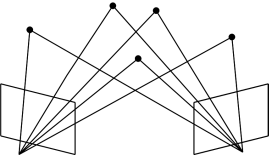
\includegraphics{5ptm2}
  \caption{Matching features in two images are projections of the same
    world point}
  \label{fig:5ptm}
\end{figure}

Features are either tracked \cite{Hedborg2009} or matched
\cite{Geiger2011} (i.e., freshly detected in each new frame) between
subsequent images. While early works chose to track features, most of
the current works detect and match them. The output of this stage are
pairs of image features, which are (hopefully) projections of the same
3D point in the real world, as in Figure~\ref{fig:5ptm}.

Matched features are used as an input for motion estimation procedure.
By whether the features are specified in 2-D or 3-D, the estimation
procedures, may be classified into 3-D-to-3-D (\cite{Milella2006},
3-D-to-2-D (\cite{Geiger2011}) and 2-D-to-2-D
(\cite{Nister2004}). Most of the early work was 3D-to-3D.  More recent
works \cite{Nister2004} claim that this approach is inferior to the
latter two. Popular techniques that participate in most algorithms in
some way are Essential matrix estimation and (possibly) its subsequent
decomposition \cite{Nister2004}, perspective 3-point algorithm
\cite{Kneip1991}, re-projection error minimization \cite{Geiger2011}.

Global methods \cite{Klein2007}, \cite{Newcombe2011} keep the map of
the environment and make sure that motion estimates are globally
consistent with this map, while local methods do not.  Some local
methods \cite{Badino2013} also keep track of (local) map , but the
underlying philosophy is different: global vs local.  Global methods
usually more accurate since they make use of a vast amount of
information (which, of course, comes at computational price).  Note
that accuracy does not imply robustness, since the outlier that made
it into the map may greatly skew subsequent pose estimates.

Methods that explicitly system state uncertainty tend to use filtering
mathematical machinery, e.g., \cite{Konolige2010}, \cite{Olson2003},
\cite{Kaess2008}.  Another alternative to maintain map/pose estimate
consistency is to use bundle adjustment approach \cite{Triggs2000}

Monocular systems \cite{Song} make use of a single camera, while
stereo systems \cite{Geiger2011} rely on a calibrated stereo rig. In
monocular setup the translation of the camera may only be estimated up
to scale, while in stereo all six motion parameters may be
recovered. Additional advantage of the stereo setup is more
information at each step, which may be one of the reasons why stereo
algorithms perform better.

\subsection{Our work}

In this work we present a novel algorithm for camera motion
estimation.  The novelty of the algorithm is in camera rotation
estimation procedure.  We rely on the fact that for scene points that
are infinitely far from the camera, the motion of the projected
(image) points may be described by a homography. For distant points
this assumption is nearly true.  Our algorithm starts by partitioning
the scene points into two sets: distant and near-by. Then, camera
Rotation is estimated from the distant points and, subsequently, the
translation is recovered from near-by points.

Current work presents the algorithm in stereo setting, however it may
also be used in monocular setting. We use stereo to partition the
scene points, in \ref{sec:mono} we discuss how this may be done in
mono.

With respect to the classification of the visual odometry methods
given in the introduction, our work is local, feature based, stereo
odometry.  We do not use bundle adjustment, however the results of our
algorithm may be subsequently improved with some form of bundle
adjustment.

The outline of the our method for two stereo image pairs:
\begin{enumerate}
\item Feature detection.  We use Harris \cite{Harris1987} features.
\item Feature matching. The matching is done both across the stereo
  pair images as well as previous vs. current pair.  We enforce
  epipolar constraint, chierality and use circle heuristics similar to
  \cite{Geiger2011} to reject outliers.
\item Partition scene points into two sets: distant and near-by.
\item Estimate camera rotation from distant points.
\item Estimate camera translation from near-by points.
\end{enumerate}

\subsection{Results Outline}

We show that on KITTI data-set our method improves upon StereoScan\cite{Geiger2011}
results and competes with state of the art methods.

\subsection{Conclusions}

\section{Preliminaries and Notation}

\subsection{Camera model}

We consider central projection of points in space onto a plane. Let
the center of projection be the origin of the euclidean frame and let
plane $Z=f$ be the image plane. World point $\mathbf{X}=[X,Y,Z]^T$ is
projected onto the image plane by means of connecting $\mathbf{X}$ and
the center of projection and taking the intersection point of the
image plane with this line to be a projected point
$\mathbf{x}=[fX/Z,fY/Z,f]^T$


If the world point is represented by a homogeneous 4-vectors, e.g.,
$\mathbf{X} = [X,Y,Z,1]^T$, then:

\begin{equation}\label{eq:central_projection}
\begin{pmatrix}
X\\ Y\\ Z\\ 1
\end{pmatrix}
\mapsto
\begin{pmatrix}
fX\\ fY\\ Z
\end{pmatrix}
=
\begin{pmatrix}
f& & &0& \\
 &f& &0& \\
 & &1&0&
\end{pmatrix}
\begin{pmatrix}
X\\ Y\\ Z\\ 1
\end{pmatrix}
\end{equation}

Equation~\ref{eq:central_projection} assumes that the origin of coordinates in
the image plane is at principal point and that the center of
projection is at the origin of the world coordinate system.

Let the coordinates of the principal point be $c = [p_x,p_y]^T$ in the
image plane frame. Also, let the camera frame orientation be described
by $R\in SO(3)$ and its origin be the inhomogeneous vector
$C\in \mathbf{R}^3$ as seen from the world frame. Thus,
Equation~\ref{eq:central_projection} becomes:

\begin{equation}\label{eq:central_projection1}
\begin{pmatrix}
X\\ Y\\ Z\\ 1
\end{pmatrix}
\mapsto
\begin{pmatrix}
fX\\ fY\\ Z
\end{pmatrix}
=
\begin{bmatrix}
f& &p_x& \\
 &f&p_y& \\
 & &1  &
\end{bmatrix}
\begin{bmatrix}
R & -RC
\end{bmatrix}
\begin{pmatrix}
X\\ Y\\ Z\\ 1
\end{pmatrix}
\end{equation}

Denote the \emph{intrinsic parameters} matrix:
\begin{equation}
\label{eq:intrinsic}
K=\begin{bmatrix} f & & p_x & \\ & f & p_y & \\ & & 1 & \end{bmatrix}
\end{equation}

Denote $\mathbf{t} = -RC$ and let the \emph{extrinsic parameters}
matrix be:
\begin{equation}
\begin{bmatrix}
R & \mathbf{t}
\end{bmatrix}
\end{equation}

Putting this together and denoting \emph{camera matrix}
$P=K[R\ \mathbf{t}]$, we may write:
\begin{equation}
\mathbf{x} = K[R\ \mathbf{t}]\mathbf{X} = P\mathbf{X}
\end{equation}

Note that, $ \mathbf{X}_{cam}= [\mathsf{R}\ \mathbf{t}]\mathbf{X}$ is the
representation of $\mathbf{X}$ in the camera reference frame.

\section{Image Point Mapping Related to Camera Motion}

Suppose the camera matrices are those of a calibrated stereo rig with
the world origin at the first camera

\[
\mathrm{P = K[I\ |\ 0]\quad P'=K'[R\ |\ \mathbf{t}]}
\]

Consider projections of a 3D point $(X,Y,Z,1)^T$ into the image planes of both views:

\[
\mathrm{\mathbf{x} = P\mathbf{X} \quad \mathbf{x}' = P'\mathbf{X}}
\]

If the image point is normalized as $\mathbf{x} = (x,y,1)^T$ then
\[
\mathbf{x}Z = \mathrm{P\mathbf{X} = K[I\ |\ 0]\mathbf{X} = K}(X,Y,Z)^T
\]

It follows that $(X,Y,Z)^T = \mathrm{K^{-1}}\mathbf{x}Z$, and:
\begin{align}
  \mathbf{x}' &= \mathrm{K'[R\ |\ \mathbf{t}]}(X,Y,Z,1)^T \\
  &= \mathrm{K'R}(X,Y,Z)^T + \mathrm{K'\mathbf{t}}\\
  &= \mathrm{K'RK^{-1}}\mathbf{x}Z + \mathrm{K'\mathbf{t}}\\
\end{align}

Now we divide both sides by $Z$ to obtain the mapping of an image point $\mathbf{x}$ to image point $\mathbf{x}'$

\begin{equation}
  \label{eq:point_motion}
  \mathbf{x}' = \mathrm{K'RK^{-1}}\mathbf{x} + \mathrm{K'}\mathbf{t}/Z = \mathrm{H}\mathbf{x}+ \mathrm{K'}\mathbf{t}/Z = \mathrm{H}\mathbf{x} + \mathbf{e'}/Z
\end{equation}

If $\mathrm{R = I}$ (e.g. pure translation) the point $\mathbf{x}$ will undergo a motion along a corresponding epipolar line:
\begin{equation}
\mathbf{x}' = \mathbf{x}+ \mathrm{K'}\mathbf{t}/Z = \mathbf{e}'/Z
\end{equation}

If $\mathbf{t} = \mathbf{0}$ the motion of the point may be represented by a homology:
\[
\mathbf{x}' = \mathrm{H}\mathbf{x}
\]

\begin{figure}[h]
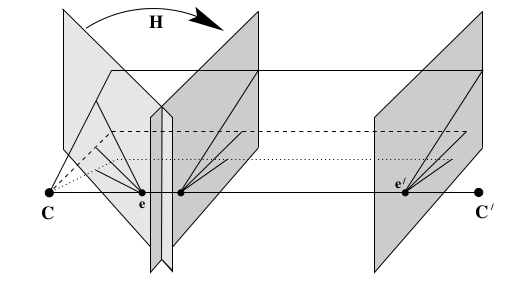
\includegraphics[scale=.3]{general_camera_motion}
\centering
\caption{General camera motion may be viewed as a two step process}
\end{figure}

In a general case the mapping of an image point $\mathbf{x}$ into $\mathbf{x}'$ may be viewed as a two step process: transformation by a homology (a specialization of homography which has two equal eigenvalues) $\mathrm{H}$ which simulates a pure rotational motion of the camera followed by an offset along the epipolar line which simulates a pure translational motion of the camera.

\section{Motion Estimation Pipeline}

\subsection{Feature Matching}
We use Harris corner detector, it is fast, well localized and corners
are abundant in urban scenes we work with. We detect corners in each
new image and then match them to obtain putative matches. We use
sum-of-square differences (SSD) as a metric function.  We enforce
epipolar and chierality (visibility) constraints for matches across a
calibrated stereo pair, thus making the search one dimensional. In a
similar fashion to \cite{Geiger2011} we enforce circular match
heuristic to prune outliers.  We tune cornerness threshold of the
detector in such a way, that we obtain about five hundred track-lets
after matching and pruning.

\subsection{Motion Estimation}
First we partition all features into two sets, distant point and
near-by points.  We do so by applying a hard threshold to the
$Z$-coordinate of the triangulated point.  This threshold is a
parameter to the algorithm and we fine-tune it using cross-validation
style procedure.

\paragraph{Rotation Estimation.} We use distant points to estimate
rotation $\mathrm{R}$. Our assumption is that for these points:

\begin{equation}
\mathbf{x}' \approx \mathrm{H}_\infty\mathbf{x} = \mathrm{K'RK^{-1}}\mathbf{x}
\end{equation}

We multiply both sides by $\mathrm{K'^{-1}}$ and denote $\mathbf{u'} = \mathrm{K'^{-1}}\mathbf{x}$ and $\mathbf{u} = \mathrm{K^{-1}}\mathbf{x}$:

\begin{equation}
\mathbf{u'} = \mathrm{K'^{-1}}\mathbf{x}' \approx \mathrm{RK^{-1}}\mathbf{x} = \mathrm{R}\mathbf{u}
\end{equation}

Since only the directions of $\mathbf{u'}$ and $\mathbf{u}$ are of
importance, we normalize them to unit length and solve absolute
orientation to obtain initial estimate of $\mathrm{R}$.

Next, we refine our estimate of $\mathrm{R}$ by means of non-linear
optimization procedure.  For each correspondence, we define its error
to be orthogonal distance to the corresponding epipolar line and
minimize the sum of squared error by means of Levenberg-Marquardt
optimization algorithm. We do so, because as \ref{eq:point_motion}
suggests after we compensate for a known rotation $\mathrm{R}$ we are
still left with (small for distant points) displacements along
epipolar lines.

To make this procedure robust to outliers, we wrap it into RANSAC
iterations.  Finally, we choose a rotation that has the largest
support set.

\paragraph{Translation Estimation} We apply translation estimation
only to near-by points.  First, we triangulate these points in the
previous stereo pair to obtain their 3-D locations, and then
iteratively minimize the sum of reprojection errors into the current
frame.

The reprojection of point $\mathbf{X}=(X,Y,Z,1)^T$ into the current
left image is given by:
\begin{equation}
  \pi^{(l)}(\mathbf{X};\mathbf{t}) =  K\Bigl[ \mathrm{R}\ |\ \mathbf{t} \Bigr]\mathbf{X} 
\end{equation}
and the reprojection of the same point into the current right image is
given by:
\begin{equation}
  \pi^{(r)}(\mathbf{X};\mathbf{t}) =  K\Bigl[ \mathrm{R}\ |\ \mathbf{t} \Bigr](\mathbf{X} - (b,0,0,0)^T)
\end{equation}
Where 
\begin{itemize}
\item $\mathrm{R}\in SO(3)$ is a rotation matrix
\item $\mathbf{t}\in \mathbf{R}^3$ is an inhomogeneous camera translation vector
\item $\mathrm{K}$ is a camera intrinsic matrix, as in \ref{eq:intrinsic}
\end{itemize}

We use Levenberg-Marquardt algorithm to iteratively minimize the sum
of squared reprojection errors:
\begin{equation}
\norm{\mathbf{x'} - \pi^{(l)}(\mathbf{X};\mathbf{t})}^2 + \norm{\mathbf{x'} - \pi^{(r)}(\mathbf{X};\mathbf{t})}^2
\end{equation}

There are three unknown parameters, since $\mathbf{t} =
(t_x,t_y,t_z)^T$, thus a single 3-D point provides enough constraints
to determine $\mathbf{t}$ (this minimization procedure is referred to
as 1-point algorithm in the literature [ref?]).

We do not search for an initial estimate of $\mathbf{t}$ since the
optimization procedure usually converges to a close enough solution.

\subsection{Monocular setting}

In this section we show how our algorithm may be adapted to monocular
setting.

The dependence of the algorithm as described in previous sections on
stereo is in the scene point partition stage.  We are interested in
points, s.t. in \ref{eq:point_motion} the $\mathbf{t}/Z$ is small
($\mathbf{t}$ is the translation of the camera or ``baseline'' and $Z$
is the depth of the 3D-point). This causes the desired property of
homography mapping to hold.

When we threshold the distance to the 3-D point (e.g., $Z$) we do it
in units of baseline, e.g.,

\begin{equation}
Z<\alpha \norm{ \mathbf{t} }
\end{equation}
which is equivalent to
\begin{equation}
\frac{\norm{\mathbf{t}}}{Z} > \frac{1}{\alpha}
\end{equation}

Note that in the monocular setting the baseline is known only up to scale, however, since $Z$ is known also up to the same scale factor.
\section{Results}

We provide results for our algorithm on a KITTI dataset
\cite{Geiger2012}.

\begin{figure}
  \centering

  \begin{minipage}[b]{0.45\linewidth}
    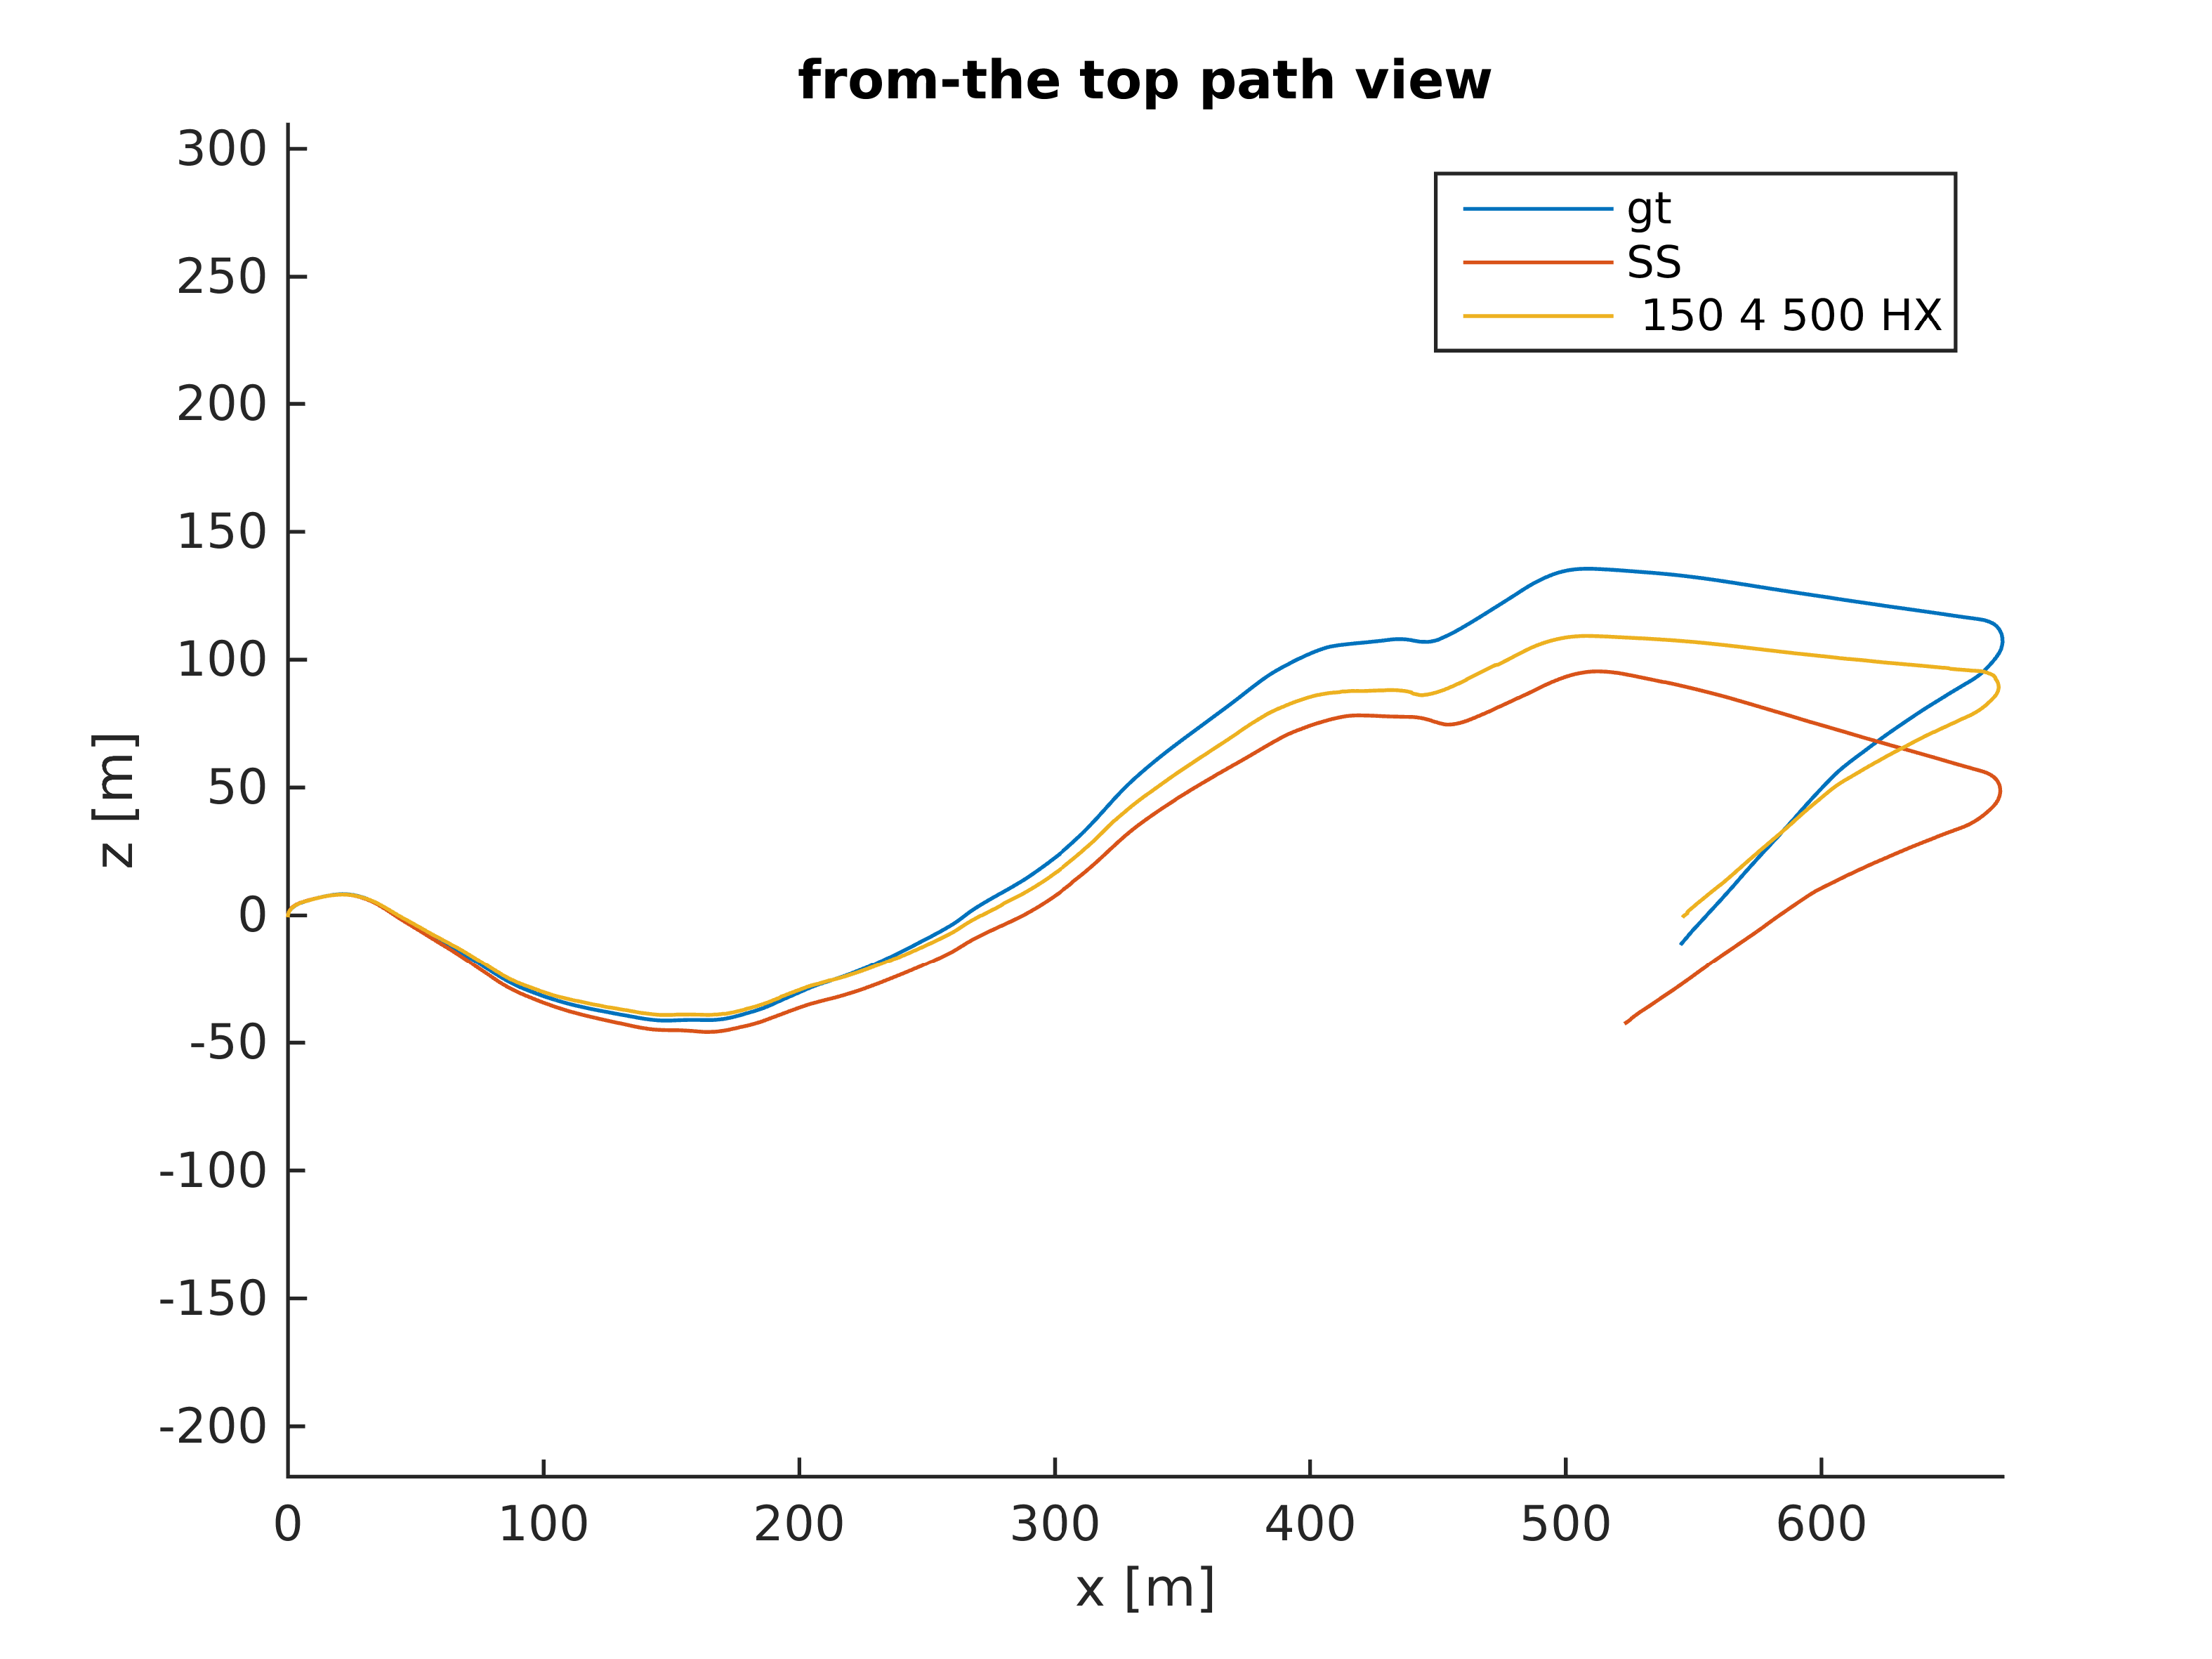
\includegraphics[scale=.4]{top_path}
    \caption{Top view of the path}
    \label{fig:4top}
  \end{minipage}
  \quad
  \begin{minipage}[b]{0.45\linewidth}
    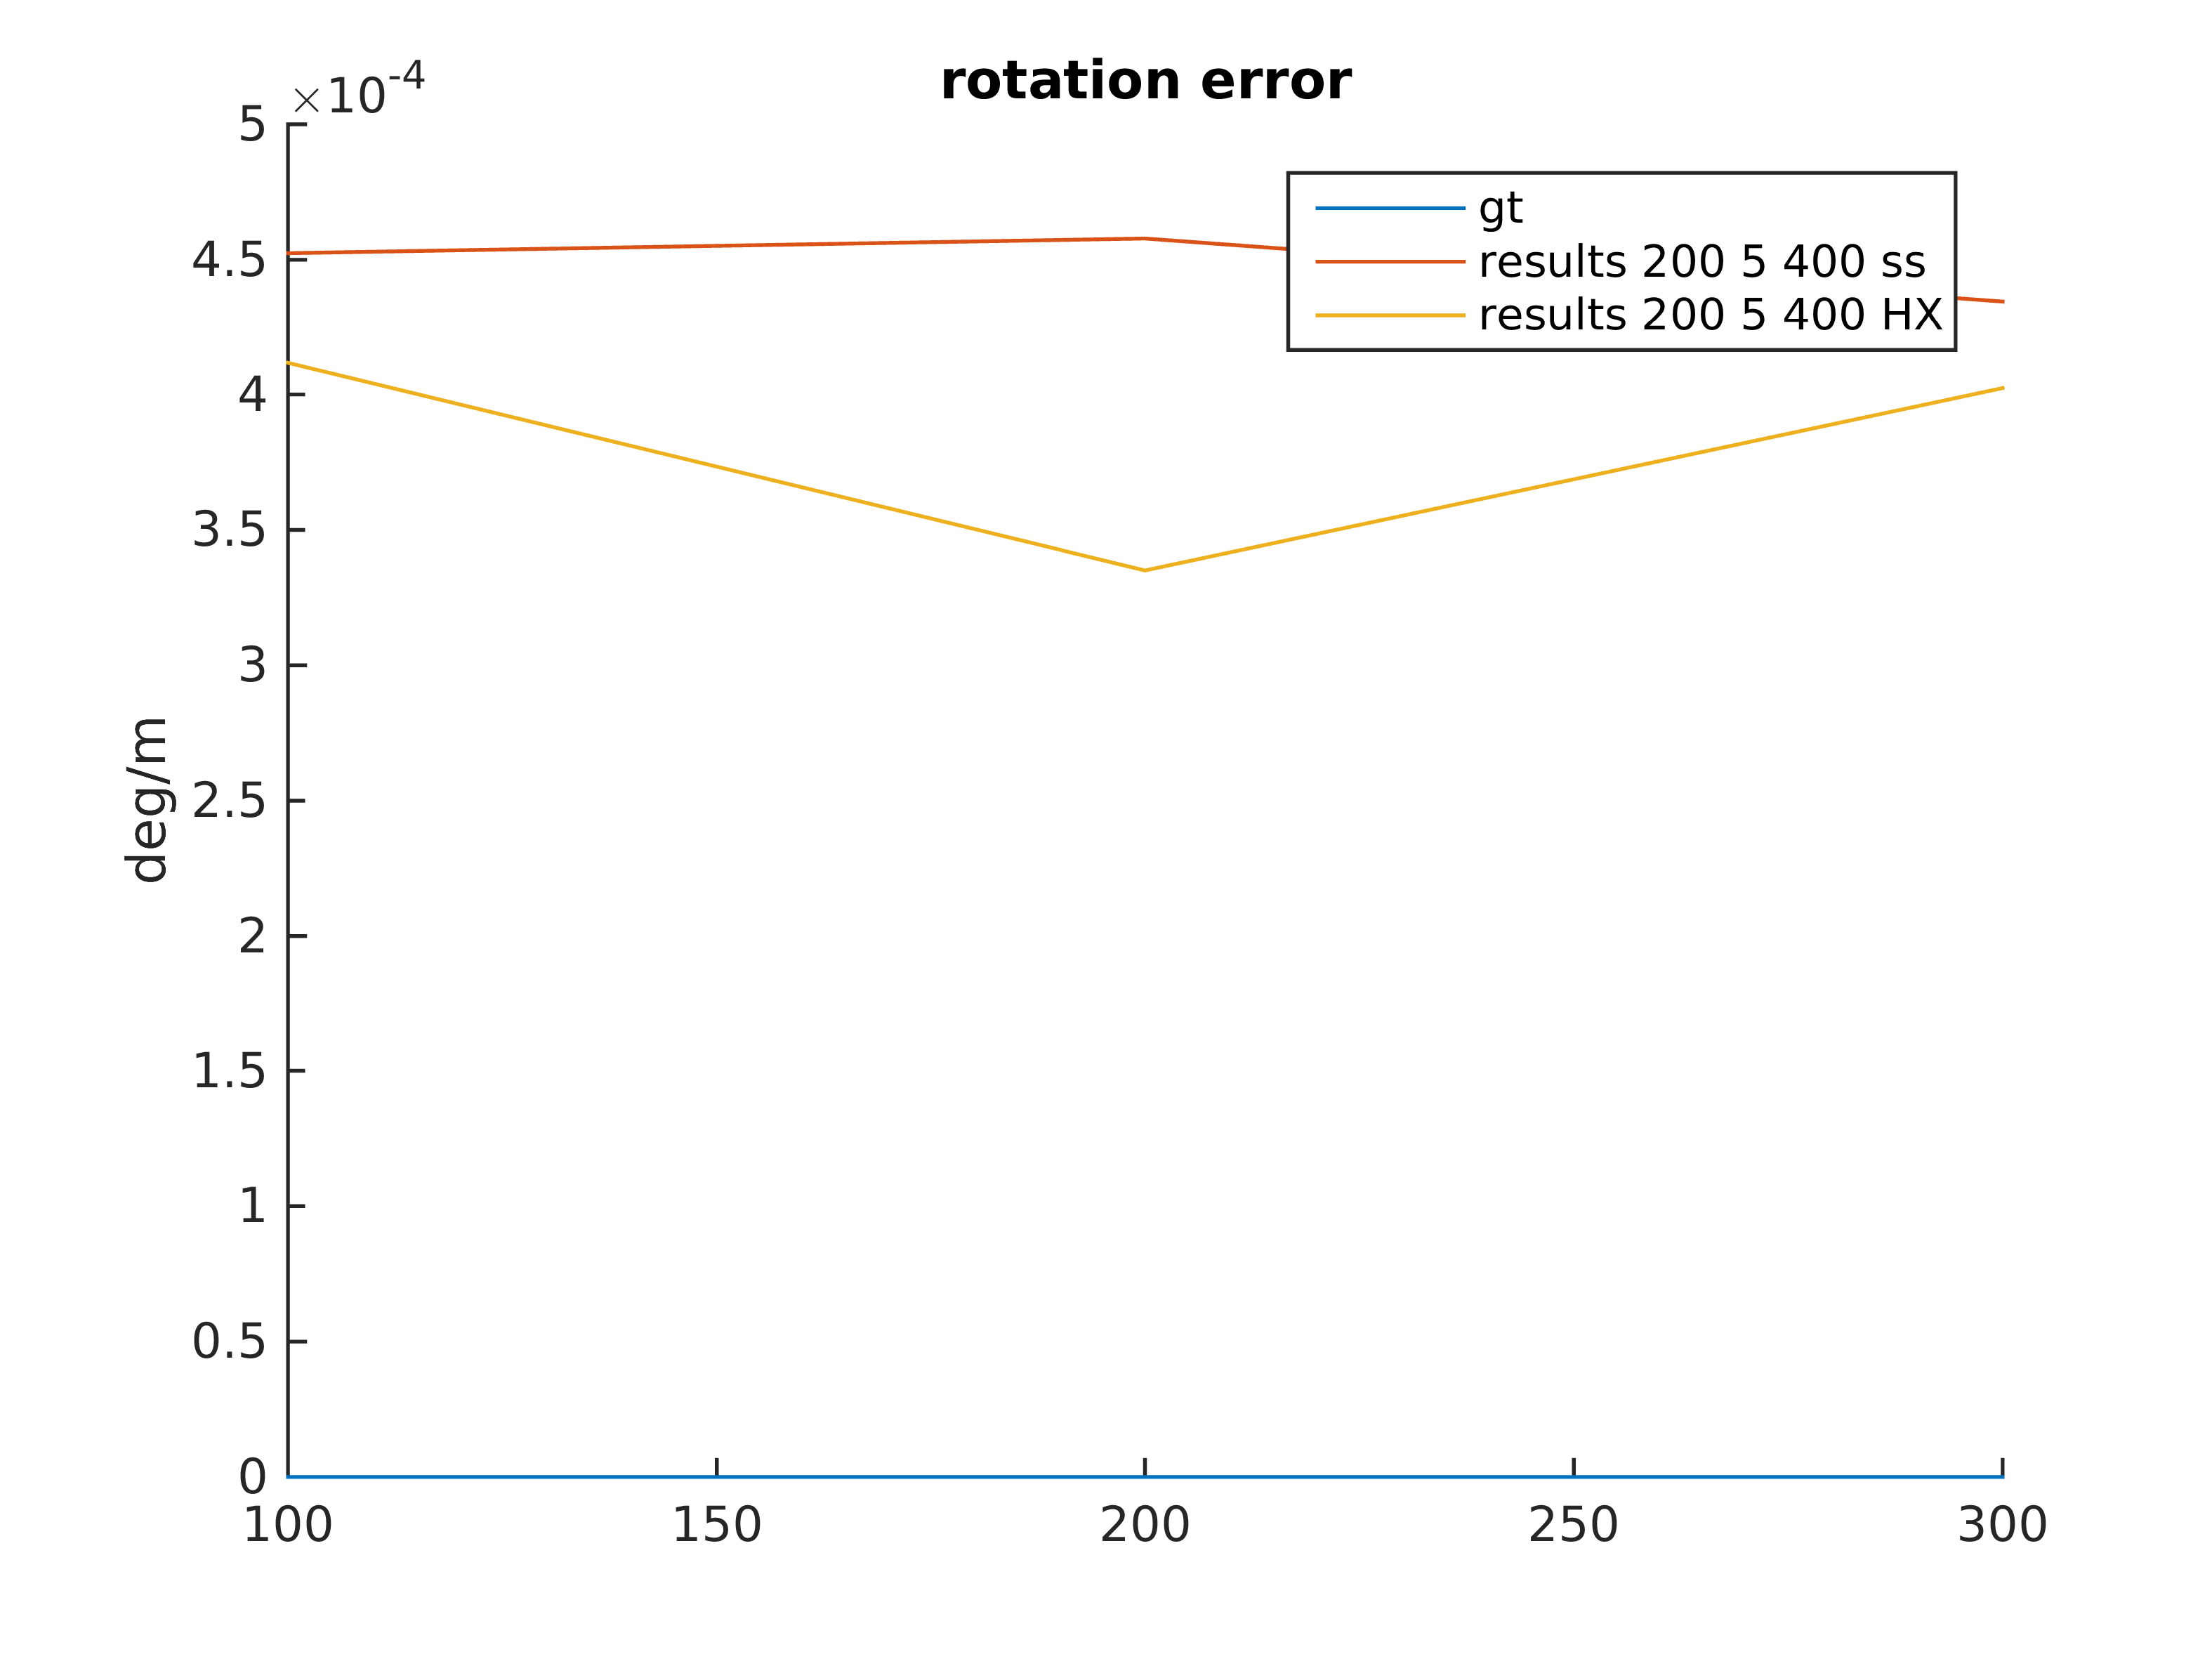
\includegraphics[scale=.4]{rotation_error}
    \caption{Rotation Error}
    \label{fig:4rot_erro}
  \end{minipage}
  \quad
  \begin{minipage}[b]{0.45\linewidth}
    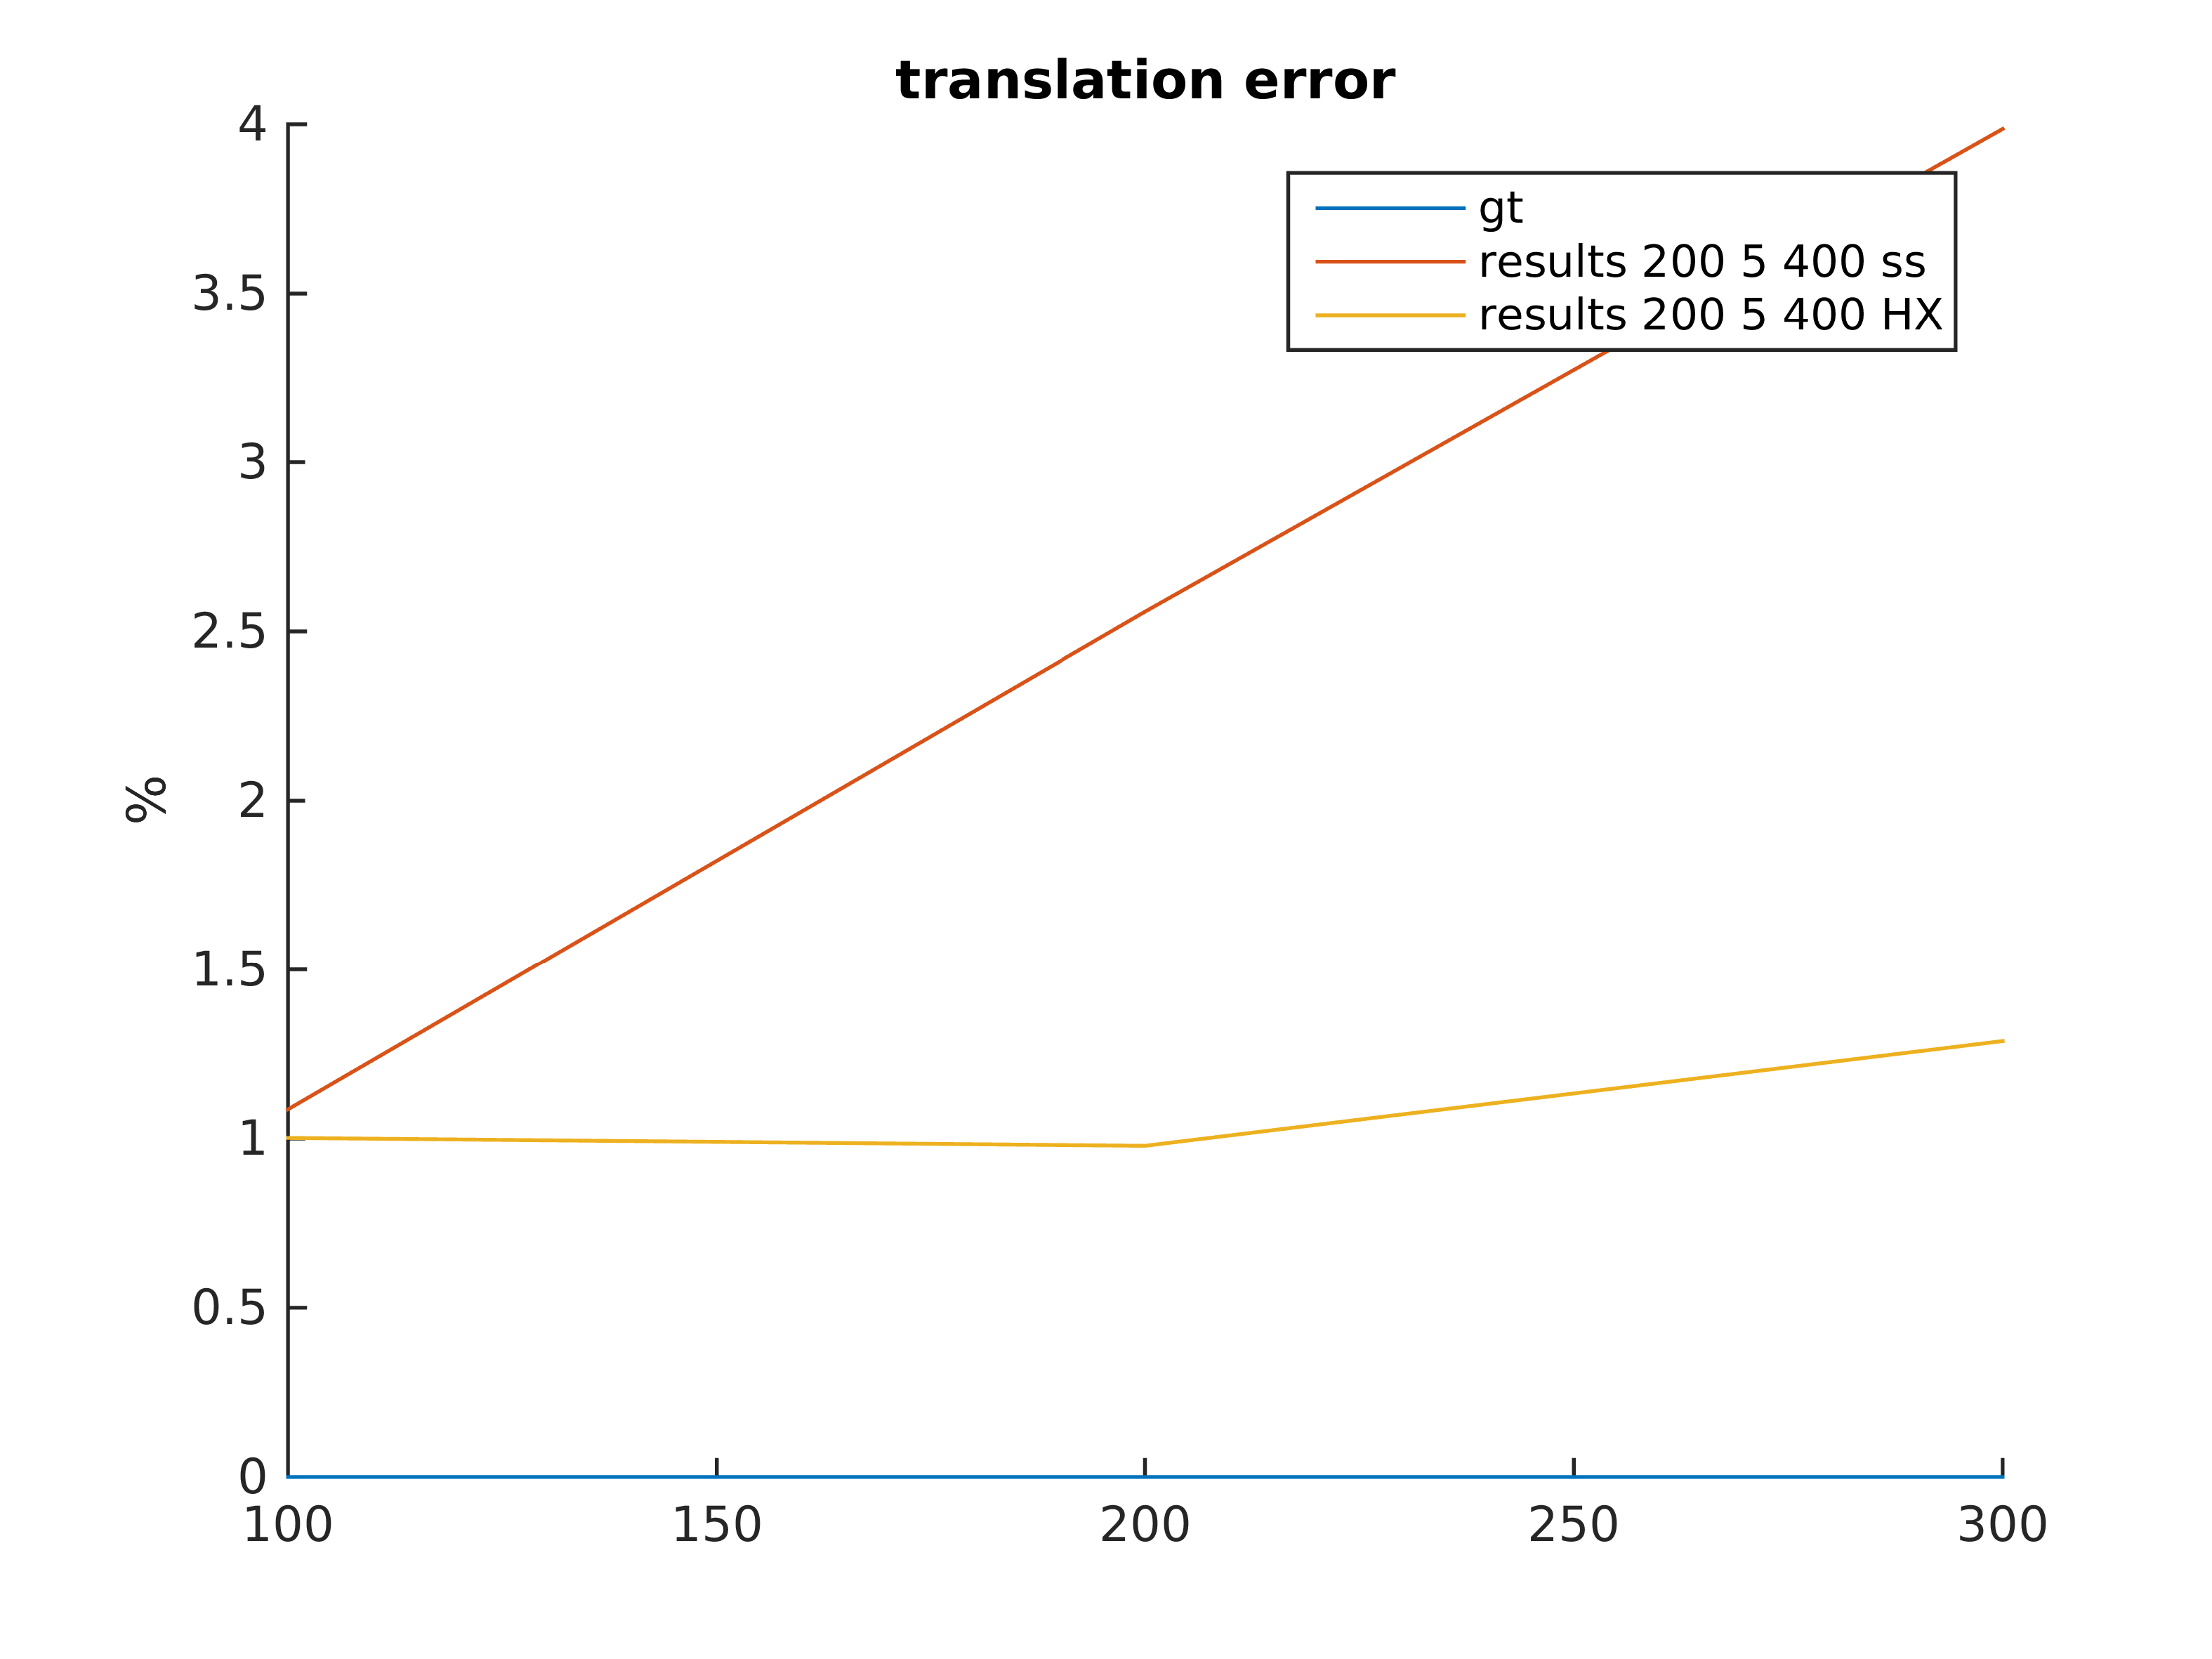
\includegraphics[scale=.4]{translation_error}
    \caption{Translation Error}
    \label{fig:4trans_error}
  \end{minipage}
\end{figure}

\clearpage\mbox{}Page \thepage\ of the manuscript.
\clearpage\mbox{}Page \thepage\ of the manuscript.
\clearpage\mbox{}Page \thepage\ of the manuscript.
\clearpage\mbox{}Page \thepage\ of the manuscript.
\clearpage\mbox{}Page \thepage\ of the manuscript.
\clearpage\mbox{}Page \thepage\ of the manuscript.
\clearpage\mbox{}Page \thepage\ of the manuscript.  This is the last
page of the manuscript.
\par\vfill\par
Now we have reached the maximum size of the ECCV 2016 submission (excluding references).
References should start immediately after the main text, but can continue on p.15 if needed.

\clearpage

\bibliographystyle{splncs}
\bibliography{egbib}
\end{document}

%%% Local Variables:
%%% mode: latex
%%% TeX-master: t
%%% End:
